\chapter{Topos theory}\label{chapter:topos}

    The main reference for this chapter is~\citet{johnstone_topos_2014,caramello_lectures_2019,caramello_topos-theoretic_2018,mac_lane_sheaves_1994}. For an introduction to stacks and descent theory, see~\citet{vistoli_notes_2004}.

    \minitoc

\section{Elementary topoi}

    \newdef{Subobject classifier}{\index{subobject!classifier}
        Consider a finitely complete category (in fact, the existence of a terminal object suffices). A subobject classifier is a mono\footnote{The symbol for this morphism will become clear in \cref{section:internal_logic}.} $\texttt{true}:1\hookrightarrow\Omega$ from the terminal object such that for every mono $\phi:x\hookrightarrow y$ there exists a unique morphism $\chi:y\rightarrow\Omega$ that fits in the following pullback square:
        \begin{figure}[ht!]
            \centering
            \begin{tikzpicture}
                \node (A) at (0, 0) {$x$};
                \node (B) at (0, -2) {$y$};
                \node (1) at (2, 0) {$1$};
                \node (O) at (2, -2) {$\Omega$};
                \node at (1, -1) {pb};
                \draw[->] (A) -- (1);
                \draw[right hook->] (A) -- node[left]{$\phi$} (B);
                \draw[right hook->] (1) -- node[right]{$\texttt{true}$} (O);
                \draw[->] (B) -- node[below]{$\exists!\chi$} (O);
            \end{tikzpicture}
            \caption{Subobject classifier.}
            \label{fig:subobject_classifier}
        \end{figure}
    }
    \begin{adefinition}
        Consider a well-powered category $\symbfsf{C}$. The assignment of subobjects $\mathrm{Sub}(x)$ to an object $x\in\ob{C}$ defines functor $\mathrm{Sub}:\symbfsf{C}^{op}\rightarrow\symbfsf{Set}$. A subobject classifier $\Omega$ is a representation of this functor, i.e.~the following isomorphism is natural in $x$:
        \begin{gather}
            \mathrm{Sub}(x)\cong\symbfsf{C}(x,\Omega)\,.
        \end{gather}
    \end{adefinition}

    \begin{example}[Indicator function]\index{indicator function}
        The category $\symbfsf{Set}$ has the 2-element set $\{\texttt{true},\texttt{false}\}$ as subobject classifier. The morphism $\chi:S\rightarrow\Omega$ is the indicator function
        \begin{gather}
            \chi_S(x)=
            \begin{cases}
                \texttt{true}&\cif x\in S\,,\\
                \texttt{false}&\cif x\not\in S\,.
            \end{cases}
        \end{gather}
    \end{example}

    \newdef{Elementary topos}{\index{topos!elementary}
        An elementary topos is a finitely complete, Cartesian closed category (\cref{cat:closed}) admitting a subobject classifier. Equivalently, one can define an elementary topos as a finitely complete category that has all power objects exist.

        The power object $Px$ of $x\in\ob{\mathcal{E}}$ is related to the subobject classifier $\Omega$ by the following relation:
        \begin{gather}
            \label{topos:power_exponential}
            Px = \Omega^x\,.
        \end{gather}
    }
    \begin{remark}[Finite colimits]
        The original definition by \textit{Lawvere} also required the existence of finite colimits. However, it can be proven that finite cocompleteness follows from the other axioms.
    \end{remark}

    \begin{theorem}[Fundamental theorem of topos theory]\index{fundamental theorem!of topos theory}
        Let $\mathcal{E}$ be an elementary topos. The slice category $\mathcal{E}_{/x}$ is also a topos for every object $x\in\ob{\mathcal{E}}$. The subobject classifier is given by $\pi_2:\Omega\times x\rightarrow x$.
    \end{theorem}

    \begin{property}[Balanced]
        All monos in a topos are regular. Hence, every mono arises as an equalizer. Since, by \cref{cat:regular_iso}, every epic equalizer is necessarily an isomorphism, it follows that every topos is balanced (\cref{cat:balanced}).
    \end{property}

    \begin{property}[Epi/mono factorization]\index{image}
        Every morphism $f:x\rightarrow y$ in a topos factorizes uniquely as an epi followed by a mono:
        \begin{gather}
            x\overset{e}{\twoheadrightarrow}z\overset{m}{\hookrightarrow}y\,.
        \end{gather}
        The mono is called the \textbf{image} of $f$.
    \end{property}

\section{Morphisms}

    \newdef{Base change}{\index{base change}\label{topos:base_change}
        Consider a category $\symbfsf{C}$ with pullbacks. For every morphism $f:x\rightarrow y$ one can define a functor $f^*:\symbfsf{C}/y\rightarrow\symbfsf{C}/x$. This functor acts by pullback along $f$.
    }
    \newdef{Dependent sum and product}{\index{dependent!sum/product}\label{topos:dependent_functors}
        Consider a base change functor $f^*$. The dependent sum and product functors are given by the right and left adjoints (if they exist):
        \begin{gather}
            \label{topos:dependent_adjoint_triple}
            \sum_f\dashv f^*\dashv \prod_f\,.
        \end{gather}
    }
    \begin{remark}
        The dependent sum can be shown to exist over any category. In fact, as a functor, it is simply given by postcomposition with $f$. However, the interpretation is much less trivial. Any morphism can be interpreted as a ``space'' with fibres the preimages. For example, in $\symbfsf{Set}$, a morphism $g:Z\rightarrow X$ represents $Z$ as follows: \[Z\cong\bigsqcup_{x\in X}g^{-1}(x)\equiv\sum_{x:X}g^{-1}(x).\] The dependent sum generalizes this construction in a fibrewise manner, i.e.~the fibre over a point $y\in Y$ is given by
        \begin{gather}
            \sum_fg\,\Big|_y = \bigsqcup_{x\in f^{-1}(y)}g^{-1}(x)\,.
        \end{gather}
        Instead of combining all fibres into a single space, it combines those that lie in a single fibre of $f$.
    \end{remark}

    Although the dependent sum always exists, the dependent product requires more structure (see e.g.~\citet{huang_locally_2022}).
    \begin{property}[Locally Cartesian closed categories]
        In a locally Cartesian closed category (\cref{cat:closed}), all dependent products exist. In fact, the existence of the adjoint triple~\eqref{topos:dependent_adjoint_triple} is equivalent to $\symbfsf{C}$ being locally Cartesian closed. For example, in $\symbfsf{Set}$, the dependent product is given by
        \begin{gather}
            \label{topos:dependent_product_sets}
            \prod_fg\,\Big|_y=\prod_{x\in f^{-1}(y)}g^{-1}(x)\,.
        \end{gather}
        When $f$ is the terminal morphism, this represents the space of sections $X\rightarrow Z\equiv\sum_{x:X}g^{-1}(x)$ of $g$.

        More generally, the functor is obtained through the product-exponential adjunction in slice categories. The pullback is equal to a product in a slice category. Since $\symbfsf{C}$ is locally Cartesian, one obtains for all $p:a\rightarrow y$ and $q:b\rightarrow y$:
        \begin{gather}
            \symbfsf{C}_{/x}(p\times f,q)\cong\symbfsf{C}_{/y}(p,q^f)
        \end{gather}
        for some morphism $q^f:b^f\rightarrow y$. Applying this exponential functor to the identity morphism $\mathbbm{1}_f$, gives a morphism $s:\mathbbm{1}_y\rightarrow f^f$ or $s:y\rightarrow x^f$ (this simply picks out the identity morphism in the exponential object internally). The dependent product is then defined as the pullback $\prod_fg:=s^*g^f$, where $g^f$ is interpreted as the morphism $(f\circ g)^f\rightarrow f^f$ in $\symbfsf{C}_{/y}$.

        The idea behind this pullback construction is that in $\symbfsf{Set}$, the pullback of $g^X:Z^X\rightarrow X^X$ along $s:\mathbbm{1}_X\rightarrow X^X$ is equal to the set
        \begin{gather}
            \{h\in Z^X\mid h\circ g=\mathbbm{1}_Z\}\,,
        \end{gather}
        i.e.~it consists of all sections of $g$. Hence, the pullback construction generalizes \cref{topos:dependent_product_sets}.
    \end{property}

    \newdef{Logical morphism}{\index{morphism!logical}
        A functor $f:\mathcal{E}\rightarrow\mathcal{F}$ between elementary topoi is said to be logical if it preserves finite limits, exponential objects and the subobject classifier.
    }
    \begin{property}
        If a logical morphism has a left adjoint if and only if it has a right adjoint.
    \end{property}

    \newdef{Geometric morphism}{\index{morphism!geometric}\index{direct!image}\index{inverse!image}
        A geometric morphism $f:\mathcal{E}\rightarrow\mathcal{F}$ of elementary topoi consists of an adjunction \[\mathcal{E}\adj{f^*}{f_*}\mathcal{F}\,,\] where the left adjoint is left exact. The right adjoint $f_*$ is called the \textbf{direct image} part of $f$ and the left adjoint $f^*$ is called the \textbf{inverse image} part. If $f^*$ itself has a left adjoint, then $f$ is said to be \textbf{essential}.
    }

    \newdef{Geometric surjection}{\index{surjective}
        A geometric morphism for which the inverse image part is faithful or, equivalently, reflects isomorphisms, is said to be \textbf{surjective} or is called a geometric surjection.
    }

    \newdef{Geometric embedding}{\index{embedding}\index{sub-!topos}\index{level}\label{topos:essential_subtopos}
        A geometric morphism for which the direct image part is fully faithful. If $\mathcal{E}\hookrightarrow\mathcal{F}$ is a geometric embedding, $\mathcal{E}$ is sometimes called a \textbf{subtopos} of $\mathcal{F}$. Moreover, if it is an essential geometric morphisms, the subtopos is itself said to be \textbf{essential}. Essential subtopoi $\mathcal{E}\hookrightarrow\mathcal{F}$ are also called \textbf{levels} of $\mathcal{F}$.
    }
    \begin{property}[Characterization of geometric embeddings]\label{topos:characterization_embedding}
        Let $f:\mathcal{E}\hookrightarrow\mathcal{F}$ be a geometric embedding and let $W\subset\mathrm{hom}(\mathcal{F})$ be the collection of morphisms that are mapped to isomorphisms under $f^*$. $\mathcal{E}$ is both equivalent to the full subcategory of $\mathcal{F}$ on $W$-local objects (\cref{cat:local_object}) and the \textit{localization} $\mathcal{F}[W^{-1}]$ at $W$ (see \cref{model:localization}).
    \end{property}

    \begin{property}[Base change]\index{base change}
        The base change functors on a topos are logical and admit a left adjoint, the postcomposition functor. This implies that these functors can be refined to essential geometric morphisms.
    \end{property}

    \begin{example}[Topological spaces]\label{topos:topological_spaces}
        Every continuous function $f:X\rightarrow Y$ induces a geometric morphism
        \begin{gather}
            \symbfsf{Sh}(X)\adj{f^*}{f_*}\symbfsf{Sh}(Y)\,,
        \end{gather}
        where the direct image functor $f_*$ is defined as
        \begin{gather}
            f_*F(U) := F(f^{-1}U)
        \end{gather}
        for any sheaf $F\in\symbfsf{Sh}(X)$ and any open subset $U\in\symbfsf{Open}(Y)$. The inverse image functor $f^*$ is defined using the equivalence between sheaves on topological spaces and \'etal\'e spaces. Consider a sheaf $E\in\symbfsf{Sh}(Y)$ as an \'etal\'e space $\pi:E\rightarrow Y$. The inverse image of $E$ along a continuous function $f:X\rightarrow Y$ is the pullback of $\pi$ along $f$.
    \end{example}

    This example implies that the global elements $\ast\rightarrow X$ of a topological space induce geometric morphisms of the form $\symbfsf{Sh}(\ast)\rightarrow\symbfsf{Sh}(X)$. By noting that $\symbfsf{Sh}(\ast)=\symbfsf{Set}$, one obtains the following generalization.
    \newdef{Point}{\index{point}
        A point of a topos $\mathcal{E}$ is a geometric morphism $\symbfsf{Set}\rightarrow\mathcal{E}$.
    }

    \newnot{Category of topoi}{
        The category of elementary topoi and geometric morphisms is a 2-category. It is denoted by $\symbfsf{Topos}$.

        To obtain the structure of a 2-category, one needs to define an appropriate notion of 2-morphism. Because a geometric morphism consists of an adjunction, one can consider two distinct conventions. Either, one can choose the 2-morphisms in $\symbfsf{Topos}$ to be the natural transformations $f^*\Rightarrow g^*$ (with associated transformations $g_*\Rightarrow f_*$) or, one can choose them to be the natural transformations $f_*\Rightarrow g_*$ (and associated transformations $g^*\Rightarrow f^*$). This chapter follows~\cite{johnstone_topos_2014} and the `inverse image convention' is used, i.e.~a 2-morphism $f\Rightarrow g$ consists of natural transformations $f^*\Rightarrow g^*$ and $g_*\Rightarrow f_*$.
    }

    \begin{property}[Balanced]
        The category $\symbfsf{Topos}$ is balanced (\cref{cat:balanced}), i.e.~every geometric morphism that is both a geometric embedding and a geometric surjection is an equivalence. 
    \end{property}

    \begin{theorem}[Factorization]\index{factorization}
        Every geometric morphisms can be factorized as a geometric surjection followed by a geometric embedding.
    \end{theorem}

\section{Internal logic}\label{section:internal_logic}

    In this subsection, finitely complete categories that admit a subobject classifier are considered (they do not have to be elementary topoi).

    \newdef{Truth value}{\index{truth value}
        A global element of the subobject classifier, i.e.~a morphism $1\rightarrow\Omega$. The subobject classifier $\Omega$ is also sometimes called the \textbf{object of truth values}.
    }

    \begin{property}[Heyting algebra]\label{topos:heyting_algebra}
        For all objects $x$ in an elementary topos, the poset of subobjects $\mathrm{Sub}(x)$ has the structure of an internal meet-semilattice since forming pullbacks of monos gives a natural transformation
        \begin{gather}
            \cap_x:\hom(x,\Omega\times\Omega)\rightarrow\hom(x,\Omega)\,.
        \end{gather}
        By the Yoneda lemma, this induces an internal map
        \begin{gather}
            \land:\Omega\times\Omega\rightarrow\Omega\,.
        \end{gather}
        In fact, it can be shown that this gives the structure of an internal Heyting algebra (\cref{set:heyting}) and, in particular, that of an internal locale (\cref{topology:locale}). Hence, every topos canonically gives an external Heyting algebra, namely $\mathrm{Sub}(1)$. Furthermore, every power object is an internal Heyting algebra. This in particular includes the subobject classifier $\Omega=P1$.
    \end{property}

    \newdef{Mitchell--B\'enabou language}{\index{Mitchell--B\'enabou language}\index{proposition}\index{type}\index{variable}\index{term}
        Let $\mathcal{E}$ be an elementary topos with subobject classifier $\Omega$.
        \begin{enumerate}
            \item\textbf{Type}: An object $x\in\ob{\mathcal{E}}$.
            \item\textbf{Variable} (of type $x$): An identity morphism $\mathbbm{1}_x$.
            \item\textbf{Term} (of type $x$ in variables $\alpha_i$ of type $x_i$): a morphism $\prod_{i\in I}x_i\rightarrow x$.
            \item\textbf{Formula} or \textbf{proposition}: a term of type $\Omega$. Moreover, a formula is deemed true if it factors through $\mathtt{true}:1\rightarrow\Omega$.
        \end{enumerate}
        The logical connectives are induced by the internal Heyting structure on $\Omega$. Quantifiers are induced by the (internal) completeness of $\Omega$.

        Every type also comes equipped with two binary relations:
        \begin{enumerate}
            \item $=_x$ is obtained from the characteristic morphism of the diagonal inclusion.
            \item $\in_x$ is obtained by using the evalution map of the exponential object together with \cref{topos:power_exponential}.
        \end{enumerate}
        Since the slices of an elementary topos are themselves elementary topoi, one can also define dependent types. An \textbf{indexed type} is an object of a slice category. \textbf{(Dependent) sums} and \textbf{products} of type families are goven by the left and right adjoints to the base change functor.
    }

    An interpretation of the Mitchell--B\'enabou language in an elementary topos $\mathcal{E}$ goes as follows.
    \newdef{Kripke--Joyal semantics}{\index{Kripke--Joyal semantics}\index{entailment}
        The \textbf{entailment} $U\vdash\phi(\alpha)$ for a term $\alpha:U\rightarrow X$ and a proposition $\phi(x):X\rightarrow\Omega$ is said to hold if $\alpha$ factors through the pullback $\{x\in X\mid\phi(x)\}$.
    }

    \begin{property}[Monotonicity]
        If $V\vdash\phi(\alpha)$ and $f:U\rightarrow V$, then $U\vdash\phi(\alpha\circ f)$.
    \end{property}
    \begin{property}[Locality]
        If $f:U\rightarrow V$ is epic and $V\vdash\phi(\alpha\circ f)$, then $U\vdash\phi(\alpha)$.
    \end{property}

\section{Grothendieck topoi}\label{section:grothendieck_topos}
\subsection{Grothendieck topologies}

    \newdef{Sieve}{\index{sieve}
        Let $\symbfsf{C}$ be a small category. A sieve $S$ on $\symbfsf{C}$ is a fully faithfull discrete fibration $S\hookrightarrow\symbfsf{C}$.

        A sieve $S$ on an object $x\in\symbfsf{C}$ is a sieve in the slice category $\symbfsf{C}_{/x}$, i.e.~$S$ is a subset of $\mathrm{ob}(\symbfsf{C}_{/x})$ closed under precomposition. In other words, if $y\rightarrow x\in S$ and $z\rightarrow y\in\mathrm{hom}(\symbfsf{C})$, then $z\rightarrow y\rightarrow x\in S$.

        All of this can be summarized by saying that a sieve on an object $x\in\ob{C}$ is a subfunctor of the hom-functor $\symbfsf{C}(-,x)$.
    }

    \begin{example}[Maximal sieve]
        Let $\symbfsf{C}$ be a category. The maximal sieve on $x\in\ob{C}$ is the collection of all morphisms $\{f\in\mathrm{hom}(\symbfsf{C})\mid\cod(f)=x\}$ or, equivalently, all of $\mathrm{ob}(\symbfsf{C}_{/x})$.
    \end{example}
    \begin{example}[Pullback sieve]
        Consider a morphism $f:x\rightarrow y$. Given a sieve $S$ on $y$, one can construct the pullback sieve $f^*S$ on $x$ as the sieve of morphisms in $S$ that factor through $f$:
        \begin{gather}
            f^*S(x) = \bigl\{g\bigm\vert f\circ g\in S(y)\bigr\}\,.
        \end{gather}
    \end{example}

    \newprop{Presheaf topos}{\index{presheaf!topos}\label{topos:presheaf_topos}
        Consider the presheaf category $\symbfsf{Psh}(\symbfsf{C})$ on an arbitrary (small) category $\symbfsf{C}$. This category is an elementary topos, where the subobject classifier assigns sieves:
        \begin{gather}
            \underline{\Omega}(x) := \{S\mid S\text{ is a sieve on }x\}\,.
        \end{gather}
        The action on a morphism $f:x\rightarrow y$ gives the morphism $\underline{\Omega}(f)$ that sends a sieve $S$ to its pullback sieve $f^*S$.

        The morphism $\texttt{true}:\underline{1}\hookrightarrow\underline{\Omega}$ is defined as the natural transformation assigning to every object its maximal sieve. For every subobject $\underline{Y}\hookrightarrow\underline{X}$ the characteristic morphism $\chi_{_{\underline{Y}}}$ is defined as follows. Consider an object $c\in\ob{C}$. The component $\chi_{_{\underline{Y}}}|_c$ is then given by
        \begin{gather}
            \chi_{_{\underline{Y}}}|_c(x) := \bigl\{f\in\symbfsf{C}(d,c)\mid\underline{X}(f)(x)\in\underline{Y}(d)\bigr\}\,,
        \end{gather}
        for all $x\in\underline{X}(c)$.
    }

    The following definition is due to \textit{Giraud} (for the original definition using the notion of a \textit{cover}, see the end of this section).
    \newdef{Grothendieck topology}{\index{Grothendieck!topology}\index{covering!sieve}\label{topos:grothendieck_topology}
        A Grothendieck topology on a category $\symbfsf{C}$ is a map $J$ assigning to every object a collection of sieves satisfying the following conditions:
        \begin{enumerate}
            \item\textbf{Identity}\footnote{The name itself stems from the fact that the maximal sieve is generated from the identity morphism.}: For every object $x\in\ob{C}$, the maximal sieve $M_x$ is an element of $J(x)$ or, equivalently, all sieves generated by isomorphisms are in $J(x)$.
            \item\textbf{Base change}: If $S\in J(x)$, then $f^*S\in J(y)$ for every morphism $f:y\rightarrow x$.
            \item\textbf{Locality}: Consider a sieve $S$ on $x\in\ob{C}$. If there exists a sieve $R\in J(x)$, such that for every morphism $(f:y\rightarrow x)\in R$ the pullback sieve $f^*S\in J(y)$, then $S\in J(x)$.
        \end{enumerate}
        The sieves in $J$ are called ($J$-)\textbf{covering sieves}. A collection of morphisms with codomain $x\in\ob{C}$ is called a \textbf{cover}\footnote{Sometimes this term is also used to denote any collection of morphism with common codomain $x$, i.e.~without reference to a covering sieve.} of $x$ if the sieve generated by these morphisms is a covering sieve on $x$.
    }

    \begin{example}[Topological spaces]
        These conditions have the following interpretation in the case of topological spaces:
        \begin{itemize}
            \item The collection of all open subsets covers a space $U$.
            \item If $\{U_i\}_{i\in I}$ covers $U$, then $\{U_i\cap V\}_{i\in I}$ covers $U\cap V$.
            \item If $\{U_i\}_{i\in I}$ covers $U$ and, if for every $i\in I$ the collection $\{U_{ij}\}_{j\in J_i}$ covers $U_i$, then $\{U_{ij}\}_{i\in I,j\in J_i}$ covers $U$.
        \end{itemize}
        The canonical Grothendieck topology on $\symbfsf{Open}(X)$ is given by the sieves $S=\{U_i\hookrightarrow U\}_{i\in I}$, where $\bigcup_{i\in I}U_i=U$. This topology is denoted by $J_{\symbfsf{Open}(X)}$.
    \end{example}

    \newdef{Site}{\index{site}
        A (small) category equipped with a Grothendieck topology $J$.
    }

    A slightly weaker notion than that of a (Grothendieck) topology is the following.
    \newdef{Coverage}{\index{coverage}\index{cover}\label{topos:coverage}
        Let $\symbfsf{C}$ be a category. A coverage on $\symbfsf{C}$ is a map that assigns to every object $x\in\ob{C}$ a collection of families $\{f:y\rightarrow x\}\subset\mathrm{hom}(\symbfsf{C})$, the \textbf{covering families} or \textbf{covers}, satisfying the following condition. If $\{f:y\rightarrow x\}$ is a covering family on $x$, then for every morphism $g:x'\rightarrow x$ there exists a covering family $\{f':y'\rightarrow x'\}$ on $x'$ such that every composite $g\circ f'$ factors through some $f$.
    }

    \newdef{Matching family}{\index{matching!family}\label{topos:matching_family}
        Consider a presheaf $F\in\symbfsf{Psh(C)}$ together with a sieve $S$ on $x\in\ob{C}$. A matching family for $S$ with respect to $F$ is a natural transformation $\alpha:S\Rightarrow F$ between $S$, regarded as a subfunctor of $\symbfsf{C}(-,x)$, and $F$.

        More explicitly, it is an assignment of an element $x_f\in Fy$ to every morphism $(f:y\rightarrow x)\in S$ such that
        \begin{gather}
            F(g)(x_f) = x_{f\circ g}
        \end{gather}
        for all morphisms $g:z\rightarrow y$. Equivalently, a matching family for $S$ with respect to $F$ is a set of elements $\{x_f\}_{f\in S}$ such that for all covering morphisms $f:y\rightarrow x,g:z\rightarrow x\in S$ and all morphisms $f':c\rightarrow y, g':c\rightarrow z$ such that $f\circ f'=g\circ g'$ the following equations holds:
        \begin{gather}
            \label{topos:matching_family_condition}
            F(f')(x_f)=F(g')(x_g)\,.
        \end{gather}
        Given such a matching family, one calls an element $a\in Fx$ an \textbf{amalgamation} if it satisfies
        \begin{gather}
            F(f)(a)=x_f
        \end{gather}
        for all morphisms $f\in S(y)$.
        
        The existence of such an element can also be stated in terms of natural transformations. Consider the obvious inclusion $\iota_S$ of $S$ into the the hom-functor $\symbfsf{C}(-,x)$. Every morphism with codomain $x$ can be obtained from the identity morphism by precomposition and, hence, a natural transformation $\symbfsf{C}(-,x)\Rightarrow F$ is determined by its action on the identity morphisms $\mathbbm{1}_x$. The existence of an amalgamation is thus equivalent to the existence of an extension of $S$ along $\iota_S$.
    }
    \remark{If the base category has all pullbacks, for example if it is a topos on its own, one can restrict the above commuting diagrams to the pullback diagrams of morphisms in the sieve $S$.}

    \newdef{Sheaf}{\index{sheaf}\index{presheaf!separated}\label{topos:sheaf}
        Consider a site $(\symbfsf{C},J)$. A presheaf $F$ on $\symbfsf{C}$ is called a $J$-sheaf if every matching family, for every covering sieve in $J$, admits a unique amalgamation\footnote{If there exists at most one amalgamation, the presheaf is said to be \textbf{separated}.} or, equivalently, if all sieves admit a unique extension to representable presheaves.

        The category $\symbfsf{Sh}(\symbfsf{C},J)$ of $J$-sheaves on the site $(\symbfsf{C},J)$ is the full subcategory of $\symbfsf{Psh(C)}$ on the presheaves that satisfy the above condition.
    }
    This definition can also be restated in terms of local objects (\cref{cat:local_object}).
    \newadef{Sheaf}{\index{descent}\label{topos:local_object_sheaf}
        By definition every covering sieve admits a morphism into the Yoneda embedding: $\eta:S\hookrightarrow\mathcal{Y}x$. If the collection of all these morphisms is denoted by $\mathcal{S}$, a presheaf is a sheaf if and only if it is $\mathcal{S}$-local, i.e.~if the following morphism is an isomorphism for all $\eta\in\mathcal{S}$:
        \begin{gather}
            Fx\cong\symbfsf{Psh}(\mathcal{Y}x,F)\xrightarrow{\symbfsf{Psh}(\eta, F)}\symbfsf{Psh}(S,F)\,.
        \end{gather}
        This is also called the \textbf{descent condition} for sheaves. In this context the collection of matching families $\mathrm{Match}(S,F):=\symbfsf{Psh}(S,F)$ for a sieve $S$ with respect to a presheaf $F$ is often called the \textbf{descent object} of $S$ with respect to $F$.
    }

    \begin{example}[Topological spaces]\index{topos!spatial}
        The usual category of sheaves $\symbfsf{Sh}(X)$ on a topological space $X$ is obtained as the category of sheaves on the site $(\symbfsf{Open}(X),J_{\symbfsf{Open}(X)})$. A Grothendieck topos of this form is also called a \textbf{spatial topos}. Since the morphisms in the covering sieves are exactly the inclusion maps $U_i\hookrightarrow U$, the pullback of two such morphisms is given by the intersection $U_i\cap U_j$. Hence, the condition for a matching family, as formulated in \cref{topos:matching_family} above, gives the second part of \cref{sheaf:def}. The uniqueness of an amalgamation is equivalent to the first part of that definition.

        For topological spaces, sheaves are easily represented visually. A matching family assigns to every set $U_i$ of an open cover $\mathcal{U}\equiv\{U_i\}_{i\in I}$ of $U$ an element $x_i\in FU_i$, such that the restrictions coincide on double overlaps, as in step $(1)$ in the figure below.
        \begin{gather*}
            \begin{tikzpicture}[baseline=-1mm]
                \node (title) at (0, 2) {Cover};
                \node (Uij) at (0, 1) {$U_i\cap U_j$};
                \node (Ui) at (-1, 0) {$U_i$};
                \node (Uj) at (1, 0) {$U_j$};
                \node (U) at (0, -1) {$U$};
                \draw[left hook->] (Uij) -- (Ui);
                \draw[right hook->] (Uij) -- (Uj);
                \draw[right hook->] (Ui) -- (U);
                \draw[left hook->] (Uj) -- (U);
            \end{tikzpicture}
            \xrightarrow{\ (1)\ }
            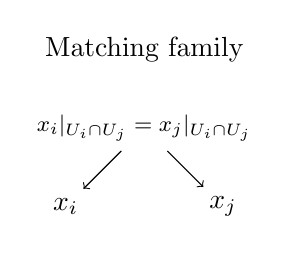
\begin{tikzpicture}[baseline=-1mm]
                \node (title) at (0, 2) {Matching family};
                \node (Uij) at (0, 1) {\footnotesize$x_i|_{U_i\cap U_j} = x_j|_{U_i\cap U_j}$};
                \node (Ui) at (-1, 0) {$x_i$};
                \node (Uj) at (1, 0) {$x_j$};
                \draw[->] (Uij) -- (Ui);
                \draw[->] (Uij) -- (Uj);
            \end{tikzpicture}
            \xrightarrow{\ (2)\ }
            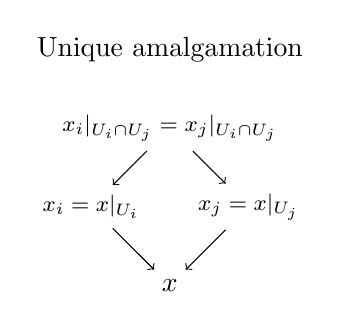
\begin{tikzpicture}[baseline=-1mm]
                \node (title) at (0, 2) {Unique amalgamation};
                \node (Uij) at (0, 1) {\footnotesize$x_i|_{U_i\cap U_j} = x_j|_{U_i\cap U_j}$};
                \node (Ui) at (-1, 0) {\footnotesize$x_i=x|_{U_i}$};
                \node (Uj) at (1, 0) {\footnotesize$x_j=x|_{U_j}$};
                \node (U) at (0, -1) {$x$};
                \draw[->] (Uij) -- (Ui);
                \draw[->] (Uij) -- (Uj);
                \draw[->] (Ui) -- (U);
                \draw[->] (Uj) -- (U);
            \end{tikzpicture}
        \end{gather*}
        The descent condition then states that for every such matching family, there exists a unique element $x$ on $U$, such that the elements of the matching family are restrictions of $x$ as in step $(2)$ of the figure above.

        The classical example would be the assignment of the set of continuous functions to open subsets of a topological space. When two functions, defined on two open sets, coincide on the intersection, there exists a unique continuous function defined on the union, such that it restricts to the given functions.
    \end{example}

    Above, in \cref{topos:coverage}, the notion of a coverage was introduced. It should be clear that every coverage generates a sieve. Furthermore, although coverages are weaker and easier to handle, they are in fact equivalent for the purpose of sheaf theory.
    \begin{property}
        Consider a covering family $C$ and let $S_C$ be the sieve it generates. A presheaf is a sheaf for $C$ if and only if it is a sheaf for $S_C$.
    \end{property}

    \begin{example}[Canonical topology]\index{topology!canonical}
        The canonical topology on a category is the finest Grothendieck topology for which all representable presheaves are sheaves. A \textbf{subcanonical topology} is then defined as a subtopology of the canonical one, i.e.~any Grothendieck topology for which all representable presheaves are sheaves.
    \end{example}
    \begin{example}[Minimal and maximal topologies]
        The minimal Grothendieck topology on a category is the one for which only the maximal sieves are covering sieves. In this topology all presheaves are sheaves. The maximal Grothendieck topology is the one for which all sieves are covering sieves. In this topology only the terminal element of the associated presheaf category is a sheaf.
    \end{example}

    \newdef{Grothendieck topos}{\index{Grothendieck|seealso{topos}}\index{topos!Grothendieck}
        A category equivalent to the category of sheaves on a (small) site. This site is often called the \textbf{site of definition} for the given topos.
    }
    \begin{property}
        Every Grothendieck topos is an elementary topos.
    \end{property}

    \begin{property}
        For every Grothendieck topos, there exists a (standard) site of definition for which the Grothendieck topology is (sub)canonical.
    \end{property}
    \begin{property}
        Let $\mathcal{E}$ be a Grothendieck topos. The canonical topology $J_{\text{can}}$ on $\mathcal{E}$ is the topology for which the covering sieves are jointly epimorphic families. Moreover,
        \begin{gather}
            \mathcal{E}\cong\symbfsf{Sh}(\mathcal{E},J_{\text{can}})\,.
        \end{gather}
    \end{property}

    \begin{construct}[Sheafification]\index{sheafification}
        Given a presheaf $\mathcal{F}$, one can construct a sheaf $\overline{\mathcal{F}}$ along the same lines of \cref{sheaf:colimit_construction}.
    \end{construct}

    \newdef{Global sections functor}{\index{global!sections}\label{topos:global_sections}
        Every Grothendieck topos $\mathcal{E}$ admits a geometric morphism to $\symbfsf{Set}$, where the right adjoint assigns to an object $x$ its set of global elements:
        \begin{gather}
            \Gamma:\mathcal{E}\rightarrow\symbfsf{Set}:x\mapsto\mathcal{E}(1,x)\,.
        \end{gather}
        When $\mathcal{E}$ is the sheaf topos over a topological space, this is exactly the global sections functor (\cref{sheaf:global_sections_functor}). The left adjoint assigns to every set $S$ the copower $S\cdot1\equiv\bigsqcup_{s\in S}1$. When $\mathcal{E}$ is a sheaf topos, this adjoint is exactly the constant sheaf functor. It is sometimes denoted by $\mathrm{LConst}$ (cf.~\cref{sheaf:constant_sheaf}).
    }

    A different approach for defining sheaf topoi is through an embedding of sheaves into presheaves.
    \newdef{Local isomorphism}{\index{local!isomorphism}
        A system of local isomorphisms in $\symbfsf{Psh(C)}$ is a class of morphisms in $\symbfsf{Psh(C)}$ forming a \textit{system of weak equivalences} (see \cref{model:weak_equivalence}) closed under pullbacks along morphisms out of representable presheaves.
    }
    \begin{property}[Local isomorphisms and Grothendieck topologies]
        A system of local isos induces a \textit{system of local epis} in the following way. $f:X\rightarrow Y$ is a local epi if $\im(f)\rightarrow Y$ is a local iso. A Grothendieck topology is defined by declaring a presheaf $F\in\symbfsf{Psh(C)}$ to be a covering sieve at $X\in\ob{C}$ if $F\hookrightarrow\mathcal{Y}X$ is a local epi.
    \end{property}

    \newadef{Sheaf topos}{\index{topos!sheaf}\label{topos:topos_geometric_embedding}
        A category $\symbfsf{Sh(C)}$ equipped with a geometric embedding into $\symbfsf{Psh(C)}$.
        \begin{mdframed}[roundcorner=10pt, linecolor=blue, linewidth=1pt]
            \begin{proof}[Proof of equivalence]
            By \cref{topos:characterization_embedding}, such a category is equivalent to the full subcategory on $S$-local presheaves for some system of local isomorphisms $S$ and, therefore, also to a sheaf topos in the sense of Grothendieck by the property above.
            \end{proof}
        \end{mdframed}
    }

    \begin{remark}[Descent condition]
        This is essentially a restatement of the descent condition (cf.~\ref{topos:local_object_sheaf}). Covering sieves, regarded as subfunctors, are in particular local isomorphisms. Stability of sieves under pullback, together with the co-Yoneda lemma~\ref{cat:ninja_yoneda}, which says that every presheaf is a colimit of representables, generates the full collection of local isomorphisms.
    \end{remark}

    The characterization of geometric embeddings and, hence, of Grothendieck topoi in terms of \textit{localizations} (\cref{topos:characterization_embedding}) is equivalent to a definition in terms of reflections (this is due to \textit{Street}).
    \begin{result}
        There exists a bijection between the Grothendieck topologies on a small category $\symbfsf{C}$ and the equivalence classes of left exact reflective subcategories of $\symbfsf{Psh(C)}$.
    \end{result}

    \newdef{Representable morphism}{\index{representable}
        A natural transformation of presheaves $F\rightarrow G$ is said to be representable if, for every representable presheaf $h_X$ and every morphism $h_X\rightarrow G$, the pullback $h_X\times_GF$ is representable.
    }

    \begin{property}[Diagonals]\label{topos:representable_diagonal}
        The diagonal morphism $\Delta_F:F\rightarrow F\times F$, for $F$ a presheaf on a category with pullbacks, is representable if and only if any of the following two equivalent properties holds:
        \begin{enumerate}
            \item For every two representable presheaves $h_X,h_Y$ and natural transformations $h_X\rightarrow F,h_Y\rightarrow F$, the pullback $h_X\times_Fh_Y$ is representable.
            \item Every natural transformation $h_X\rightarrow F$ from a representable presheaf is representable.
        \end{enumerate}
    \end{property}

\subsection{Topological sheaves}

    See \cref{chapter:sheaf} for the application of sheaves to topology.

    \begin{property}[Presheaf topos]\label{topos:sheaf_topos}
        Consider the presheaf category
        \begin{gather}
            \symbfsf{Psh}(X):=\symbfsf{Psh\bigl(Open}(X)\bigr)
        \end{gather}
        over a topological space $(X,\tau)$. Unpacking \cref{topos:presheaf_topos} shows that this category is an elementary topos where the subobject classifier is given by
        \begin{gather}
            \Omega(U) = \{V\in\tau\mid V\subseteq U\}\,.
        \end{gather}
    \end{property}

    \begin{construct}[Sheaves and \'etale bundles]\index{bundle}\label{topos:etale_adjunction}
        Let $X$ be a topological space. The functor
        \begin{gather}
            I:\symbfsf{Open}(X)\rightarrow\symbfsf{Top}_{/X}:U\mapsto(U\hookrightarrow X)
        \end{gather}
        induces the following adjunction:
        \begin{gather}
            \symbfsf{Top}_{/X}\adj{E}{\Gamma}\symbfsf{Psh}(X)\,.
        \end{gather}
        The slice category on the left-hand side is the category of (topological) \textit{bundles} (see \cref{chapter:bundles}) over $X$. Both directions of the adjunction have a clear interpretation. The right adjoint assigns to every bundle its sheaf of local sections and the left adjoint assigns to every presheaf its bundle of germs.

        By restricting to the subcategories on which this adjunction becomes an adjoint equivalence, one obtains the \textbf{\'etale space} and \textbf{sheaf categories} respectively:
        \begin{gather}
            \symbfsf{Et}(X)\cong\symbfsf{Sh}(X)\,.
        \end{gather}
        The category on the right-hand side is the category of sheaves on a topological space $X$. The category on the left is the full subcategory on local homeomorphisms, i.e.~the \'etale spaces (\cref{topology:etale_space}).
    \end{construct}

    \begin{property}[Associated sheaf]
        The inclusion functor $\symbfsf{Sh}(X)\hookrightarrow\symbfsf{Psh}(X)$ admits a left adjoint, the \textbf{sheafification functor}, that assigns to every presheaf its associated sheaf. This functor is given by the composition $\Gamma\circ E$, which is simply \cref{sheaf:etale_construction}.

        The fact that the counit of the adjunction (\cref{topos:etale_adjunction}) restricts to an isomorphism on the full subcategory $\symbfsf{Sh}(X)$ is equivalent to the fact that the sheafification of a sheaf $\Gamma$ is again $\Gamma$.
    \end{property}

    \newdef{Petit and gros topoi\footnotemark}{\index{topos!petit \& gros}\index{topos!spatial}
        \footnotetext{For those that do not master French, `\textit{petit}' and `\textit{gros}' mean small and big, respectively.}
        Consider a topological space $X$ together with its category of opens $\symbfsf{Open}(X)$. The petit topos over $X$ is defined as the sheaf topos $\symbfsf{Sh}(X)\equiv\symbfsf{Sh}\bigl(\symbfsf{Open}(X)\bigr)$. It represents $X$ as a `generalized space'. (By \cref{topos:etale_adjunction}, the objects in a petit topos are the \'etale spaces over the given base space.) Topoi equivalent to such petit topoi are sometimes said to be \textbf{spatial}. However, one can also build a topos whose objects are themselves generalized spaces. To this end, choose a site $S$ of `probes' and call the sheaf topos $\symbfsf{Sh}(S)$ a gros topos. (See \cref{section:smooth_spaces} for more information.)
    }

    \begin{property}[Localic reflection]\index{localic!reflection}
        Mapping a topological space to its sheaf of continuous sections defines a functor $\func{\symbfsf{Sh}}{Top}{Topos}$ by \cref{topos:topological_spaces}. When restricted to the full subcategory of sober spaces (\cref{topology:sober_space}), this functor becomes fully faithful. Generalizing to locales even gives a reflective inclusion (\cref{cat:reflective_inclusion}).

        This property states that no information is lost when regarding (sober) topological spaces as sheaf topoi. This also explains the name `petit topos'.
    \end{property}

    \newdef{Localic topos}{\index{localic!topos}
        Multiple equivalent definitions exist:
        \begin{enumerate}
            \item A topos equivalent to a sheaf topos over a locale (\cref{topology:locale}) equipped with the topology of jointly surjective morphisms.
            \item A topos generated under colimits of subobjects of the terminal object $1$.
            \item A topos $\mathcal{E}$ for which the global sections functor $\Gamma:\mathcal{E}\rightarrow\symbfsf{Set}$ is localic, i.e.~every object in $\mathcal{E}$ is a subquotient of an object in the inverse image $\Gamma^*$
        \end{enumerate}
        Given a geometric morphism to some base topos $\mathcal{S}$, one can define $\mathcal{S}$-localic topoi by generalizing the third point.
    }
    The following property shows that the locale in the first definition has a specific meaning.
    \begin{property}
        By \cref{topos:heyting_algebra}, for every topos the poset $\mathrm{Sub}(1)$ is a locale. Every localic topos $\mathcal{E}$ satisfies $\mathcal{E}\cong\mathrm{Sh}\bigl(\mathrm{Sub}(1)\bigr)$, where $\mathrm{Sub}(1)$ is equipped with the topology of jointly surjective morphisms.
    \end{property}

    The equivalence between localic topoi and locales carries over to the notion of $\mathcal{S}$-localic topoi.
    \begin{property}
        The (2-)category of localic topoi over a base topos $\mathcal{S}$ is equivalent to the (2-)category $\symbfsf{Loc}(\mathcal{S})$ of locales internal to $\mathcal{S}$.
    \end{property}
    \begin{property}\label{topos:slice_locale}
        Given a locale $X$, the category $\symbfsf{Loc}\bigl(\symbfsf{Sh}(X)\bigr)$ is equivalent to the slice category $\symbfsf{Loc}_{/X}$.
    \end{property}

\subsection{Lawvere--Tierney topology}

    This section gives an alternative approach to the construction of sheaf topoi, which is more closely linked to the logical aspect of topos theory.

    \newdef{Lawvere--Tierney topology}{\index{Lawvere--Tierney}
        As noted in \cref{section:internal_logic} on the internal logic of elementary topoi, the subobject classifier $\Omega$ has the structure of an internal Heyting algebra and, in particular, that of a (bounded) meet-semilattice. This internal poset, viewed as an internal category, admits the construction of a closure operator $j:\Omega\rightarrow\Omega$ (\cref{cat:closure_operator}) satisfying the following condition:
        \begin{gather}
            j\circ\land = \land\circ(j\times j)\,.
        \end{gather}
        This condition states (in a nontrivial way) that $j$ is (internally) order-preserving. More concisely, a Lawvere--Tierney topology is internally a left exact modality on $\Omega$.
    }
    \begin{remark}
        The condition satisfied by the unit morphism in the definition of a closure operator can also be reformulated in this context as follows:
        \begin{gather}
            j\circ\texttt{true} = \texttt{true}\,.
        \end{gather}
    \end{remark}

    \begin{example}[Double negation topology]\index{topology!double negation}\label{topos:double_negation}
        As mentioned above, the subobject classifier in an elementary topos has the structure of an internal Heyting algebra and, hence, admits a negation morphism $\lnot:\Omega\rightarrow\Omega$. It can be shown that double negation $\lnot\lnot:\Omega\rightarrow\Omega$ gives a Lawvere--Tierney topology.
    \end{example}
    \begin{property}\index{Booleanization}\index{Boolean!subtopos}\index{dense!subtopos}
        The Booleanization $\mathcal{E}_{\lnot\lnot}\hookrightarrow\mathcal{E}$ of an elementary subtopos is the smallest dense subtopos of $\mathcal{E}$ and the largest Boolean subtopos of $\mathcal{E}$, i.e.~it is the unique subtopos such that:
        \begin{enumerate}
            \item\textbf{Dense}: $\mathcal{E}_{\lnot\lnot}$ contains the initial object $\bot$.
            \item\textbf{Boolean}: $\Omega$ is a Boolean algebra.
        \end{enumerate}
    \end{property}
    
    As noted above, Lawvere--Tierney operators induce, internally, \textit{universal closure operators} on all posets $\mathrm{Sub}(x)$ in the topos. Given an object $x$ and a subobject $u\in\text{Sub}(x)$, one defines the closure $j_\ast(u)\in\text{Sub}(x)$ as the subobject classified by the characteristic morphism $j\circ\chi_u:x\rightarrow\Omega$.
    \newdef{Dense object}{\index{dense}\index{closed}
        Given a Lawvere--Tierney topology $j:\Omega\rightarrow\Omega$, a subobject $u\in\text{Sub}(x)$ is said to be dense (in $x$) if it satisfies $j_\ast(u)\cong x$. An object is said to be \textbf{closed} if $j_\ast(u)\cong u$.
    }

    \begin{example}
        On a presheaf topos, objects are dense exactly if they are covering sieves (\cref{topos:grothendieck_topology}).
    \end{example}

    The following definition allows to generalize sheaves from topoi to finitely complete categories.
    \newadef{Sheaf}{\index{sheaf}\index{separated}
        Given a Lawvere--Tierney topology $j:\Omega\rightarrow\Omega$ on a topos $\mathcal{E}$, one calls an object $s\in\ob{\mathcal{E}}$ a $j$-sheaf if it is local with respect to all dense morphisms (\cref{cat:local_object}), i.e.~for all dense morphisms $u\hookrightarrow x$ the induced map \[\mathcal{E}(x,s)\rightarrow\mathcal{E}(u,s)\] is a bijection. If this map is only a monomorphism, the object is said to be \textbf{$j$-separated}.
    }

    \begin{property}\index{sheafification}
        Lawvere--Tierney topologies on $\mathcal{E}$ are in correspondence with subtopoi of $\mathcal{E}$, given by the sheaves relative to the chosen topology. As before, the left adjoint to the embedding is the sheafification functor.
    \end{property}

    In the case of (pre)sheaf topoi, Lawvere--Tierney topologies recover Grothendieck topologies.
    \begin{result}
        For the presheaf topos on a small category $\symbfsf{C}$, the Grothendieck topologies on $\symbfsf{C}$ are equivalent to Lawvere--Tierney topologies on $\symbfsf{Psh(C)}$.
        \begin{mdframed}[roundcorner=10pt, linecolor=blue, linewidth=1pt]
            \begin{proof}[Sketch of proof]
                Since a Grothendieck topology assigns to every object a collection of sieves, \cref{topos:presheaf_topos} implies that $J(x)\subseteq\Omega_{\symbfsf{Psh}}(x)$ for all $x\in\ob{C}$. By the base change condition of Grothendieck topologies, this relation is natural in $x$ and, hence, $J$ is a subobject of $\Omega_{\symbfsf{Psh}}$. One thus finds a characteristic morphism $j:\Omega_{\symbfsf{Psh}}\rightarrow\Omega_{\symbfsf{Psh}}$ that can be proven (by the other conditions of Grothendieck topologies) to define a Lawvere--Tierney topology on $\symbfsf{Psh(C)}$. Conversely, a Lawvere--Tierney topology is a morphism $j:\Omega\rightarrow\Omega$ and, hence, determines a unique subobject of $\Omega_{\symbfsf{Psh}}$, i.e.~a unique collection of sieves for every object $x\in\ob{C}$. From the conditions of Lawvere--Tierney topologies, one can then prove that this collection satisfies the conditions of a Grothendieck topology.
            \end{proof}
        \end{mdframed}
    \end{result}

\subsection{Diaconescu's theorem}\label{section:diaconescu}\index{Diaconescu}

    The following concept weakens the notion of left exact functors to categories where not all (finite) limits exist.
    \newdef{Flat functor}{\index{flat!functor}\label{topos:flat_functor}
        A functor $\func{F}{C}{Set}$ is said to be flat if the opposite of the category of elements $\mathrm{El}(F)^{\text{op}}$ (\cref{cat:category_of_elements}) is filtered (\cref{cat:filtered}). The category of flat functors on $\symbfsf{C}$ is denoted by $\symbfsf{Flat}(\symbfsf{C},\symbfsf{Set})$.

        A general functor $\func{F}{C}{D}$ is said to be \textbf{(representably) flat} if, for every object $d\in\ob{D}$, the opposite comma category $(d/F)^{\text{op}}$, which is equivalently the opposite category of elements $\mathrm{El}\bigl(\symbfsf{D}(d,-)\circ F\bigr)^{\text{op}}$, is filtered.
    }

    The definitions above can be stated more explicitly as follows (cf.~\cref{cat:finitely_complete_alternative}). The functor $\func{F}{C}{D}$ is representably flat if for every $d\in\ob{D}$:
    \begin{enumerate}
        \item There is at least one object $c\in\ob{C}$ and a morphism $f:d\rightarrow Fc$. Hence, at least one inhabited set in the image of $F$.
        \item For every two objects $c,c'\in\ob{C}$ and every two morphisms $f\in\symbfsf{D}(d,Fc)$ and $g\in\symbfsf{D}(d,Fc')$, there exists an object $x\in\ob{C}$ and morphisms $i\in\symbfsf{C}(x,c)$, $j\in\symbfsf{C}(x,c')$ and $h\in\symbfsf{D}(d,Fx)$ such that $Fi\circ h=f$ and $Fj\circ h=g$.
        \item For every two parallel morphisms $f,g\in\symbfsf{C}(c,c')$ and morphism $h\in\symbfsf{D}(d,Fc)$ such that $Ff\circ h=Fg\circ h$, there exists a morphism $i\in\symbfsf{C}(x,c)$ and a morphism $j\in\symbfsf{D}(d,Fx)$ such that $f\circ i=g\circ i$ and $Fi\circ j=h$.
    \end{enumerate}

    \begin{remark}
        Note that flatness and representable flatness are only equivalent for $\symbfsf{Set}$-valued functors when the domain $\symbfsf{C}$ is finitely complete.
    \end{remark}

    \begin{property}\index{Yoneda!extension}
        Consider the \textbf{Yoneda extension} that maps a functor $F\in\funccat{C}{Set}$ to a functor $\widetilde{F}:\cfunccat{C}{Set}\rightarrow\symbfsf{Set}$ through left Kan extension along the Yoneda embedding. $F$ is flat if and only if $\widetilde{F}$ is left exact.\footnote{By \cref{cat:kan_extension_alternative}, Kan extensions admit an expression is terms of adjoints. In this setting, the right adjoint has the form of a Hom-functor and, accordingly, the Yoneda extension is sometimes written as a tensor product $-\otimes_{\symbfsf{C}}F$. The terminology `flat' is then in analogy with \cref{homalg:flat_module}. This essentially coincides with the tensor product of functors \cref{cat:copower_product}.}
    \end{property}
    \begin{property}\label{topos:flat_or_ind}
        A functor $\func{F}{C}{Set}$ is flat if and only if it is the filtered colimit of representable functors or, equivalently, if $F$-weighted filtered colimits commute with finite limits. Note that, by \cref{cat:pro_object_uproperty}, this means that
        \begin{gather}
            \symbfsf{Flat(\op{C},Set)}\cong\symbfsf{Ind(C)}\,.
        \end{gather}
    \end{property}

    The previous property implies the following statement, which is the $\symbfsf{Set}$-valued version of \textit{Diaconescu's theorem}, which will be covered in its internal version below.
    \begin{theorem}[Diaconescu: Set version]
        A functor $\func{F}{C}{Set}$ is flat if and only if the induced adjunction $\symbfsf{Set}\leftrightarrows\cfunccat{C}{Set}$ is a geometric morphism or, alternatively, if flat functors are equivalent to global points of the presheaf topos $\cfunccat{C}{Set}$.
    \end{theorem}

    \newdef{Morphism of sites}{\index{morphism!of sites}
        A representably flat functor preserving covers.
    }

    Now, for $\mathcal{E}$ a cocomplete topos, a functor $\func{F}{C}{\mathcal{E}}$ is said to be \textbf{(internally) flat} if it representably flat with respect to the internal logic of $\mathcal{E}$ or, equivalently, if the Yoneda extension $\mathrm{Lan}_{\mathcal{Y}}F$ is left exact.
    \begin{property}\index{flat!functor}
        A functor $\func{F}{C}{\mathcal{E}}$, with $\mathcal{E}$ a cocomplete topllos, is flat if and only if:
        \begin{itemize}
            \item The family of terminal morphisms in $\symbfsf{C}$ is jointly epimorphic.
            \item For all $c,d\in\ob{C}$, the family of morphisms into $Ac\times Ad$ induced by spans $c\leftarrow b\rightarrow d$ is jointly epimorphic.
            \item For any two parallel morphisms $f,g$ in $\symbfsf{C}$, the family of factorizations of morphisms through their equalizer is jointly epimorphic.
        \end{itemize}
        These conditions are equivalent to the following ones:
        \begin{itemize}
            \item For every object $x\in\mathcal{E}$, there exists a jointly epimorphic family $\{x_i\rightarrow x\}_{i\in I}$ and and a family $\{x_i\rightarrow F(c_i)\mid c_i\in\ob{C}\}_{i\in I}$.
            \item For all $c,d\in\ob{C}$ and generalized elements $\lambda:x\rightarrow Fc\times Fd$, there exists an epimorphic family $\{\lambda_i:x_i\rightarrow x\}_{i\in I}$ and a family of spans $\{c\xleftarrow{f}b_i\xrightarrow{g}d\}_{i\in I}$ equipped with a family of generalized elements $\{\kappa_i:x_i\rightarrow Fb_i\}_{i\in I}$ such that
            \begin{gather}
                (Ff,Fg)\circ\kappa_i = \lambda\circ\lambda_i\,.
            \end{gather}
            \item For any two parallel morphisms $f,g:c\rightarrow d$ in $\symbfsf{C}$ and any generalized element $\lambda:x\rightarrow Fc$ such that $Ff\circ\lambda=Fg\circ\lambda$, there exists an epimorphic family $\{\lambda_i:x_i\rightarrow x\}_{i\in I}$ and families of morphisms $\{f_i:c_i\rightarrow c\}$ and $\{\kappa_i:x_i\rightarrow Fc_i\}$ such that
            \begin{gather}
                \begin{aligned}
                    f\circ f_i &= g\circ f_i\\
                    Ff_i\circ\kappa_i &= \lambda\circ\lambda_i
                \end{aligned}
            \end{gather}
            for all $i\in I$.
        \end{itemize}
    \end{property}

    \begin{theorem}[Diaconescu: Topos version]
        Consider a cocomplete topoi $\mathcal{E}$ and a (small) category $\symbfsf{C}$. There exists an equivalence
        \begin{gather}
            \symbfsf{Topos}\bigl(\mathcal{E},[\symbfsf{C}^{\mathrm{op}},\symbfsf{Set}]\bigr)\leftrightarrows\symbfsf{Flat}(\symbfsf{C},\mathcal{E})\,,
        \end{gather}
        where
        \begin{itemize}
            \item flat functors are sent to geometric morphisms whose inverse image part is given by left Kan extension along the Yoneda embedding and direct image part is given by:
            \begin{gather}
                F\mapsto\bigl(x\mapsto\mathcal{E}(F-, x)\bigr)\,,
            \end{gather}
            and
            \item geometric morphisms are sent to the precomposition of the inverse image part with the Yoneda embedding.
        \end{itemize}
    \end{theorem}

    To pass to the internal logic of topoi, \cref{cat:filtered} needs to be generalized to internal category theory (\cref{section:internal_category_theory}).
    \newdef{Internally filtered category}{\index{category!filtered}
        An internal category $\symbfsf{C}\in\symbfsf{Cat}(\mathcal{E})$ satisfying:\footnote{Some sources require all these morphisms to be regular epis.}
        \begin{enumerate}
            \item The terminal morphism $C_0\twoheadrightarrow1$ is an epi.
            \item For any two generalized elements $\lambda_1,\lambda_2:U\rightarrow C_0$, there is an epi $\theta:V\twoheadrightarrow U$ and corresponding $V$-elements $\gamma_1,\gamma_2:V\rightarrow C_0$ such that
            \begin{gather}
                \begin{aligned}
                    d_1\circ\gamma_1 &= d_1\circ\gamma_2\\
                    d_0\circ\gamma_i &= \lambda_i\circ\theta
                \end{aligned}
            \end{gather}
            for $i=1,2$.
            \item For any two parallel generalized elements $\gamma_1,\gamma_2:U\rightarrow C_1$ such that $d_0\circ\gamma_1=d_0\circ\gamma_2$, there exists an epi $\theta:V\twoheadrightarrow U$ and a $V$-element $\kappa:V\rightarrow C_1$ such that
            \begin{gather}
                \begin{aligned}
                    d_1\circ\kappa &= d_0\circ\lambda_1\circ\theta = d_0\circ\lambda_2\circ\theta\\
                    c(\kappa,\lambda_1\circ\theta) &= c(\kappa,\lambda_2\circ\theta)\,.
                \end{aligned}
            \end{gather}
        \end{enumerate}
    }